\section{Installing \SM}
\label{InstallationSection}
\SM's source code is stored in a CVS repository at
\url{cvs.cs.arizona.edu}. You can get the source
anonymously (in which case you can't make
any changes to it):
To get the sources anonymously, do the following
\begin{verbatim}
   > setenv CVS_RSH ssh
   > cvs -d :pserver:anonymous@cvs.cs.arizona.edu:/cvs/wmark login
   > cvs -d :pserver:anonymous@cvs.cs.arizona.edu:/cvs/wmark \
      checkout -P smark3 smextern3 smapps3 smbloat3 smbin3 smtest3
\end{verbatim}
or, if you have write access to \SM\ (i.e an account on 
\url{cvs.cs.arizona.edu}) you should instead do 
\begin{verbatim}
   > setenv CVS_RSH ssh
   > cvs -d :ext:MyLogin@cvs.cs.arizona.edu:/cvs/cvs/wmark \
          checkout -P smark3 smextern3 smapps3 smbloat3 smbin3 smtest3
\end{verbatim}
where {\tt MyLogin} is your account name on \url{cvs.cs.arizona.edu}.

You should now have four directories:
\begin{description}
  \item[smark3:]     The SandMark sources.
  \item[smbin3:]     Scripts.
  \item[smextern3:]  External Java code i.e. jar and zip files
                    needed to run SandMark.
  \item[smapps3:]    Some simple applications you can use to try
                    out SandMark
  \item[smbloat3:]   Some simple test cases for Bloat. Read these
                    to get a feel for how Bloat should be used.
  \item[smtest3:]    A test suite for SandMark.
\end{description}

Once you have checked out \SM\ you can get the latest
version by running the {\tt cvs update} command:
\begin{verbatim}
   > cd smark3
   > cvs update -dP
\end{verbatim}
To add a new file you do {\tt cvs add file}, to remove it
{\tt cvs rm file} and to commit your changes to the
repository at \url{cvs.cs.arizona.edu} you say 
{\tt cvs commit}.

\subsection{Building \SM}
Note that you will need Java 1.4 to run SandMark properly.
Get the latest version from \url{http://java.sun.com/j2se/1.4}.

Do the following to build \SM:
\begin{verbatim}
> cp smark3/Makedefs.std smark3/Makedefs
# Make the 'obvious' changes to Makedefs.
# In particular, you should set these variables:
#   JDK =
#   HOME = 

> cp smbin3/smark.std smbin3/smark
# Make the 'obvious' changes to smark.
# Again, you should set these variables:
#   JDK =
#   HOME = 

> cp smapps3/Makedefs.std smapps3/Makedefs
# Make the same obvious changes as in smark3/Makedefs

> make -C smark3

# Build applications to watermark
> make -C smapps3

# Start SandMark
> ./smbin3/smark
\end{verbatim}

\SM\ gets compiled into a jar-file \url{sandmark.jar}.
To execute it you also need some other packages ({\tt bloat},
{\tt BCEL}, etc.), which can be found in the {\tt smextern}
directory. The {\tt smark} script takes care of setting
Java's classpath correctly so that these get picked up.

You can verify that SandMark works using the test suite:

\begin{verbatim}
# Set some environment variables.
# The current directory should contain
# smtest3, smark3, smextern3, etc.
> export SMEXTERN=$PWD/smextern3/
> export SMJAR=$PWD/smark3/sandmark.jar

# JDK_ROOT should contain bin/, lib/, jre/
# and other stuff
> export JDK_ROOT=/path/to/jdk/

# run the test script
> ./smtest3/bin/runtests
\end{verbatim}

See smtest3/README for details of how to add and remove tests.

You can also build the manual:
\begin{verbatim}
> make -C smark3/doc/ manuals.ps
> make -C smark3/doc/ manuals.ps
\end{verbatim}

Finally, you can generate html from the JavaDoc
comments in the source:
\begin{verbatim}
> make -C smark3 jdoc
\end{verbatim}
This generates a directory \url{jdoc} of html files.

A minimal installation of SandMark contains 5 files:
sandmark.jar, bloat-1.0.jar, BCEL.jar, grappa1\_2.jar, 
and smark3.  bloat-1.0.jar, BCEL.jar, and grappa1\_2.jar
should all be in a directory called smextern3, sandmark.jar
should be in a directory called smark3, and these 2 
directories should have the same parent directory.  smark3
can have any path.

\section{SandMark in Windows}
To run SandMark in Windows, a minimal installation is necessary, along
with a java runtime environment version 1.4.0 or greater.  Before running
SandMark, you must set the environment variable CLASSPATH (case insensitive
in Windows) to include the path of sandmark.jar BCEL.jar and bloat-1.0.jar.
The image below shows the dialog to set user environment variables in
Windows XP.

%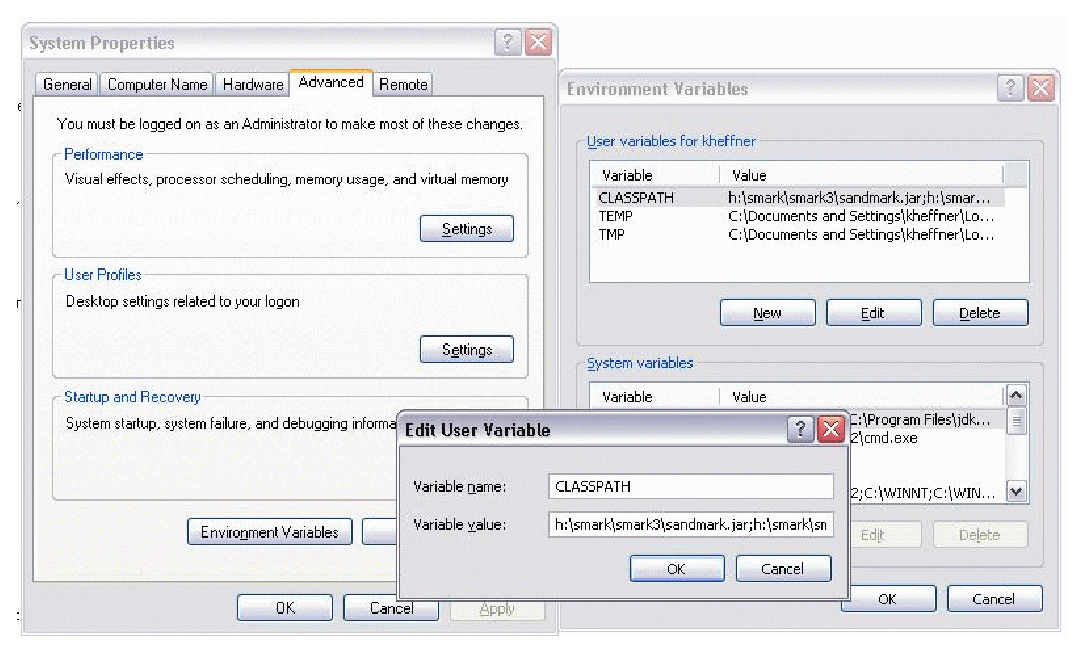
\includegraphics{figs/windows.eps}

Each path in the classpath is seperated by a semicolon.  Once the 
environment variables are set, to run SandMark, open a command 
prompt window (Start Menu $\rightarrow$ Run, and type in \verb/command/ and
press enter) and type \verb/java sandmark.Console/.
